\documentclass[runningheads]{llncs}
\usepackage{graphicx}
\begin{document}
\begin{titlepage}
\centering
{\scshape\LARGE University of Potsdam \par}
\vspace{1cm}
{\scshape\Large Project in Computational Intelligence\par}
\vspace{1.5cm}
{\huge\bfseries Merging Robot Plans in the asprilo framework\par}
\vspace{2cm}
{\Large\itshape Adrian Salewsky\par}
\vfill
supervised by\par
Etienne Tignon
\vfill
{23.03.2021 \par}


\begin{abstract}
This paper shows my approach to solving the plan merging problem in multi-agent path finding. This means that plans for single robots are combined to a plan for all robots. During the merging, all arising conflicts must be dealt with. This was done for a project
at the University of Potsdam in the course Computational Intelligence for the chair Computational Intelligence. The project was done in the asprilo framework with the programming language Answer Set Programming. 
\end{abstract}
\end{titlepage}


\section{Introduction}
The multi-agent path finding (MAPF) problem deals with multiple agents that have to find their way to a goal. This paper deals with the problem of having plans for single robots and combining them to a plan that contains all robots. During the merging of the plans, arising conflicts must be solved. The solution presented in this paper uses the asprilo framework by potassco \cite{asprilo}, the language Answer Set Programming (ASP) and the solver clingo 5.4.0. More details on the asprilo framework will be given in the next section. Section 3 contains my idea on how to theoretically solve the plan merging problem. In the section after that, I will show my ASP encoding. Sections 5 and 6 contain the analysis of my solution as well as comparing my approach to approaches of other groups that have worked on the same problem. I will end my paper with a conclusion. My solution as well as the used benchmarks can be found in my github repository \cite{owngithub}.


\section{The asprilo framework}
The asprilo framework deals with robots in a warehouse. The framework has several domains. The ``M-Domain'' is the one that simplifies the problem to MAPF. The goal is that at the last time step (called horizon) all shelves containing an ordered product have a robot under them. This is done by finding plans for the robots in which they move to a shelf in the designated time. The asprilo framework uses ASP. This means the plans are created by using predicates and rules. The predicate stating when and how a robot moves is $move(R,D,T)$ with R being the robot, D being the direction it moves in and T being the time step at which the robot moves. To track the positions of robots the predicate $position(R,C,T)$ is used. R is the robot again, C is the node the robot is positioned on and T is the time step again. The $position$ predicate is also used for shelves. The resulting plan is shown in the form $occurs(object(robot,R),action(move,D),T)$. The arguments are the same as in the $move$ predicate. It is simply another form of representing them. \\
There is also a visualizer for this framework. It is used to see how the found solution works. Images shown in this paper are screenshots taken from the visualizer.
Since the plan merging problem uses the plans of single robots, the asprilo framework was used to create these plans. The visualizer was used to verify the correctness of the solutions.


\section{Idea}
The main idea behind my solution is that every time a conflict arises, one of the robots participating in the conflict randomly changes its movement during that time step and pushes his original plan back. 
To do that, the program needs to detect the conflicts and choose a robot who has to solve the conflict by generating a new move. The problem that arises is that
there is no option to overwrite predicates in ASP. Therefore, a new argument was needed for every predicate describing a plan. This new argument is called $conflict\_nr$ and 
the higher this argument is in a predicate the newer is the plan containing that predicate. This idea is a very simple approach to solving the problem since it completely adapts the original plan and only
inserts additional moves. This way the resulting solution might not have an optimal move set for every robot but it should be able to theoretically solve most problem instances. 

\section{Answer Set Programming Encoding}
\subsection{Pre-Required Predicates}
To solve the problem, there are several predicates needed before starting to solve the conflicts. There are two domain intervals whose upper bounds are constants: $time$, which states at which time step something happens, with the constant $horizon$ and $conflict\_nr$, which states how many conflicts have been solved to reach this plan, with the constant $c\_nr$.
The constants are chosen at run-time. \\ There are some predicates that have been taken over from the encoding for the asprilo framework: $isRobot(robot(R))$ to check if something is a robot, $position((X,Y))$ to check if the node (X,Y) exists, $direction((X,Y))$ declares the 4 directions a robot can go into and $nextto(C1,D,C2)$ states that you get from the node C1 to the node C2 if you move into direction D. \\  
As input, the program expects a plan of the form $occurs(object(robot,R),action(move,D),T)$. This is transformed into the predicate $move(R,D,T,0)$. This means that the original plan has the $conflict\_nr$ 0. \\
Another part that has been mostly taken over from the encoding for the framework itself is the declaration of the position predicates:
\begin{verbatim}
position(R,C,0,0) :- init(object(robot,R), value(at,C)).
position(R,C,T,A) :- move(R,D,T,A), position(R,C',T-1,A), nextto(C',D,C).
                  :- move(R,D,T,A), position(R,C ,T-1,A), not nextto(C ,D,_).
position(R,C,T,A) :- position(R,C,T-1,A), not move(R,_,T,A), conflict_nr(A), 
                     isRobot(robot(R)), time(T).
\end{verbatim}
The difference is that position also contains an argument A for the $conflict\_nr$. The position only gets changed if a move in the same conflict depth A exists. The inertia rule also got changed accordingly. \\
The last part needed before the conflict solving is the predicate $goal$:
\begin{verbatim}
goal(R,C) :- position(R,C,horizon,0).
:- position(R,C,horizon,_), goal(R,C'), C!=C'.
\end{verbatim}
These rules declare that the last position of the initial plan is the goal position and that there can be no plan where a robot
is not on its goal position at the end. While this does not change the solution itself (the plan always only gets pushed back so the robot always ends on the same node), it improves the solution time. \\


\subsection{Conflict Detection and Selection}
There are two types of conflicts that can appear in a problem instance. The first one is that a robot arrives on a node which is either already occupied by another robot or another robot arrives in the same time step (see figures \ref{fig:c1_1} and \ref{fig:c1_2}).

\begin{figure}
   \begin{minipage}[b]{.4\linewidth} 
      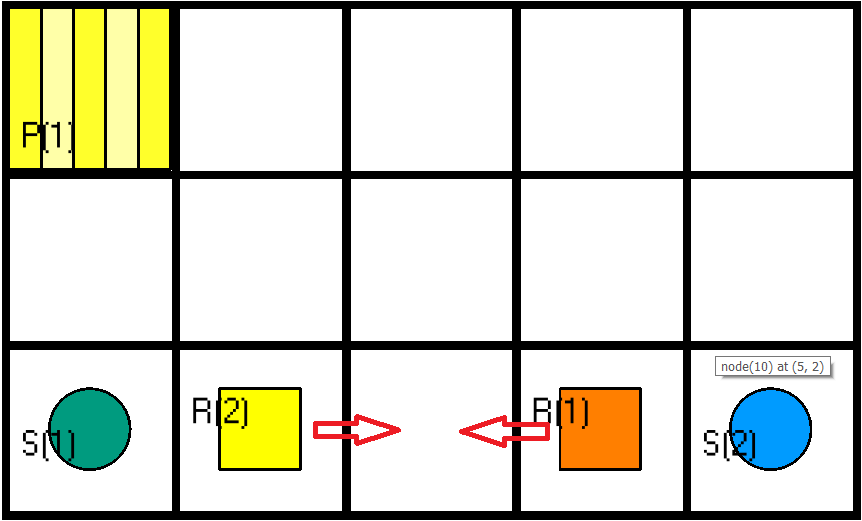
\includegraphics[width=\linewidth]{Images/Conflict 1_1}
      \caption{Two robots arrive on the same node at the same time step.}
      \label{fig:c1_1}
   \end{minipage}
   \hspace{.1\linewidth}
   \begin{minipage}[b]{.4\linewidth} 
      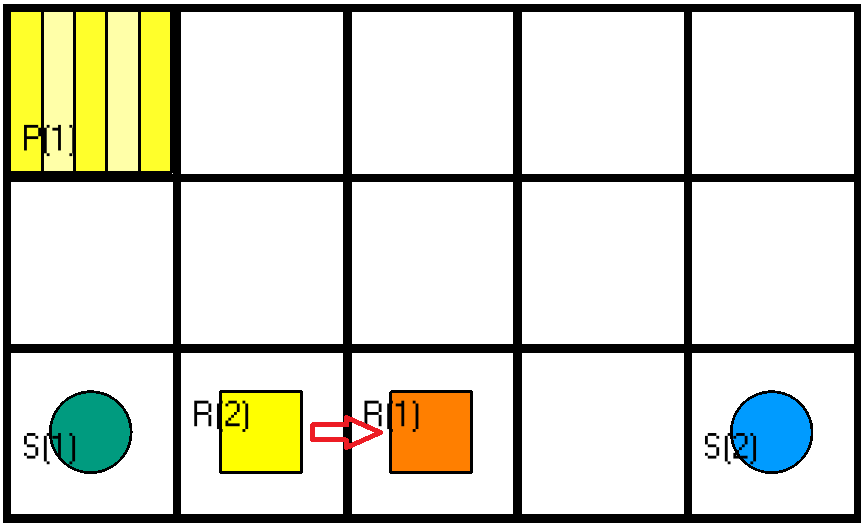
\includegraphics[width=\linewidth]{Images/Conflict 1_2}
      \caption{A robot moves to an already occupied node.}
      \label{fig:c1_2}
   \end{minipage}
\end{figure} 

\begin{verbatim}
conflict(R1,T,A) :- position(R1,C1,T-1,A), position(R1,C2,T,A), 
                    position(R2,C2,T,A), R1!=R2, conflict_nr(A).
\end{verbatim}
The predicate $conflict(R,T,A)$ is derived for the two robots participating in the conflict. \\
The second conflict is two robots switching their places (see figure \ref{fig:c2}):

\begin{figure}[h]
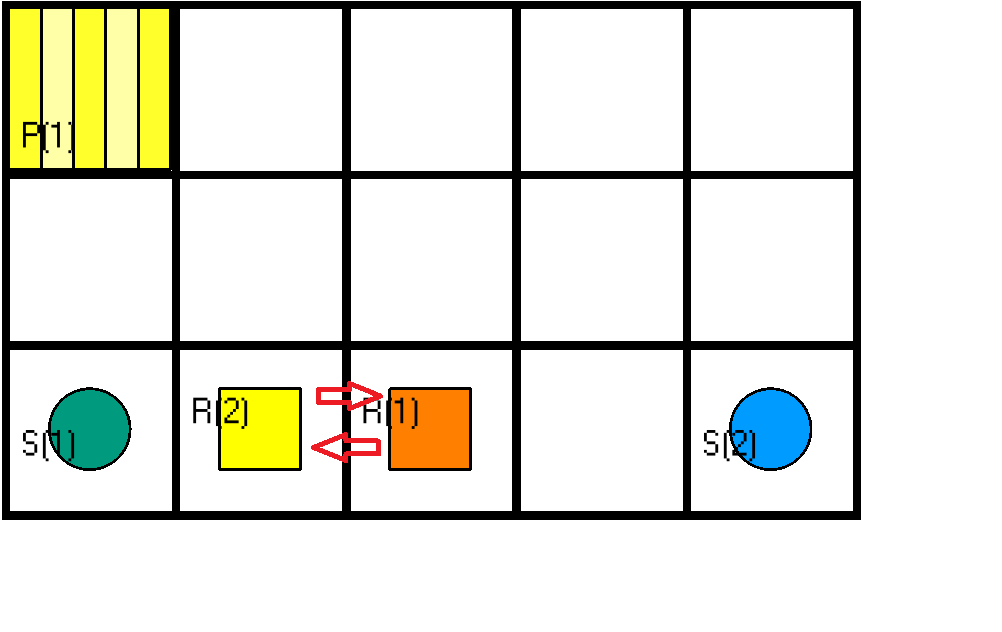
\includegraphics[width=75mm]{Images/Conflict 2}
\caption{Two robots switch places.}
\label{fig:c2}
\end{figure}

\begin{verbatim}
conflict(R1,T,A) :- position(R1,C1,T-1,A), position(R1,C2,T,A), 
                    position(R2,C2,T-1,A), position(R2,C1,T,A), 
                    R1!=R2, conflict_nr(A).
\end{verbatim}
The same predicate is derived for this type of conflict. \\
The program detects all of the conflicts arising in a plan this way. Only one conflict can get solved in each conflict depth, otherwise multiple plans get created for each robot because there would be separate plans to solve each conflict. The program chooses one of the conflicts that appeared the earliest.
\begin{verbatim}
1{solving_conflict(R,T,A) : conflict(R,T,A)}1 :- conflict(_,_,A).
:- conflict(_,T,A), solving_conflict(_,T',A), T'>T.
\end{verbatim}
The first rule declares that one conflict is chosen as the $solving\_conflict$ in each conflict depth. The second rule declares that a conflict cannot be chosen as solving conflict if there is a conflict that appears in an earlier time step in the same conflict depth. \\
This conflict selection makes it completely random which robot gets chosen as the one who has to solve the conflict. This could mean that the solver finds a plan where a lot of conflicts arise because of inefficient robot selection. This is why I have chosen to let the solver minimize the number of the conflicts:
\begin{verbatim}
#minimize {1,(R,T,A): solving_conflict(R,T,A)}.
\end{verbatim}
This rules forces the solver to find the most efficient way of selecting robots for the conflict solving.

\subsection{Conflict Solving}
After a robot is chosen as the conflict solver, its plan gets changed. 
\begin{verbatim}
0{move(R,D,T,A+1) : direction(D), nextto(C,D,_)}1 :- 
                  solving_conflict(R,T,A), position(R,C,T-1,A).
\end{verbatim}
The solver either chooses that the robot has to wait for this time step or that it moves into a random direction.
In both cases the $conflict\_nr$ has to rise for all robots:
\begin{verbatim}
position(R,C,T-1,A+1) :- solving_conflict(R',T,A), isRobot(robot(R)),
                         position(R,C,T-1,A).
move(R,D,T',A+1) :- solving_conflict(R',T,A), isRobot(robot(R)), R!=R', 
                    move(R,D,T',A), T'>=T.
\end{verbatim}
The first rule raises the conflict depth of the position predicate of every robot in the time step before the conflict. The second rule raises the conflict depth of every move predicate of every robot, except the selected one, in every time step after the conflict. This way only the predicates starting from the time step of the conflict get changed. This reduces the amount of predicates compared to always changing all the predicates including the ones before the conflict happened. \\
The only thing left is to change the plan of the selected robot accordingly. Since there are two possible solutions for a conflict, there are two ways to push back the plan. The first possible solution is that the robot waits. In this case the plan only needs to get pushed back by one time step:
\begin{verbatim}
move(R,D,T'+1,A+1) :- solving_conflict(R,T,A), not move(R,_,T,A+1), 
                      move(R,D,T',A), T'>=T, time(T').
\end{verbatim}
The second possibility is that the robot moves into a random direction. If this is the case, the robot has to move into the opposite direction to be able to reach its goal position. The problem is that it is hard to decide at which time step the robot goes back since there could be new problems if it moves back at a time where there is already an occupied node which creates new conflicts. This is why, I let the solver decide at which time step the robot moves back:
\begin{verbatim}
1{step_back(R,(DX',DY'),T_B,A+1) : time(T_B), T_B<=horizon, T_B>T}1:- 
        solving_conflict(R,T,A), move(R,(DX,DY),T,A+1), DX'=-DX, DY'=-DY.
\end{verbatim}
This rule chooses a time step between the conflict and the horizon where the robot moves into the opposite direction of the dodge move. After that, the plan of the robot gets raised in conflict depth while changing the time steps accordingly:
\begin{verbatim}
move(R,D,T,A) :- step_back(R,D,T,A).
move(R,D,T'+1,A+1) :- solving_conflict(R,T,A), step_back(R,_,T_B,A+1), 
                      move(R,D,T',A), T'>=T, T<T_B-1.
move(R,D,T'+2,A+1) :- step_back(R,_,T_B,A+1), move(R,D,T',A), T'>=T_B-1.
\end{verbatim}
Since there are two rules in which the solver randomly decides which action to take, it is of advantage again to let the solver minimize the arising conflicts. This way the chosen actions result in the smallest number of conflicts.

\subsection{Integrity Constraints}
There are several integrity constraints used to ensure the correctness of the program as well as reducing the solution time.
These constraints only check if the predicates move out of the domain:
\begin{verbatim}
:- move(_,_,T,_), T>horizon.
:- position(_,_,T,_), T>horizon.
:- move(_,_,_,A), A>c_nr.
:- position (_,_,_,A), A>c_nr.
:- conflict(_,T,_), T>=horizon.
:- conflict(_,_,A), A>=c_nr.
\end{verbatim}
The conflict predicate cannot have $horizon$ or $c\_nr$ itself as argument because if a conflict arises the plan needs to get changed again and the predicates would move out of bounds.


\subsection{Output}
The resulting plan should only take the predicate with the highest conflict depth in each time step. 
\begin{verbatim}
new_move(R,D,T) :- move(R,D,T,MAX_C), MAX_C == #max{A: position(R,C,T-1,A)}.
\end{verbatim}
The predicate $new\_move$ contains the moves that had the highest conflict depth. The highest conflict depth is determined by looking at the position before a move. Every time a conflict arises, the position before the conflict has its conflict depth raised. This means that the position predicate is always the latest. The move predicate cannot be used to determine the highest conflict depth because there is no move predicate if a robot is waiting. \\
The predicate $new\_move$ gets translated into a form resembling the original input:
\begin{verbatim}
new_occurs(object(robot,R),action(move,D),T) :- new_move(R,D,T).
\end{verbatim}
The solver shows the $new\_occurs$ predicates as its solution.

\subsection{Extra Features}
There are two extra features I have dealt with. The first extra feature is the possibility of declaring that certain robots do not have to change their plan at all.
This is done by adding the predicate $strict\_plan(R\_ID)$ with $R\_ID$ being the ID of a robot. The only thing that gets changed in the encoding is in the conflict detection part:
\begin{verbatim}
conflict(R1,T,A) :- position(R1,C1,T-1,A), position(R1,C2,T,A), position(R2,C2,T,A), 
                    R1!=R2, conflict_nr(A), not strict_plan(R1).
\end{verbatim}
The only things that gets added is that a robot can only have a conflict that it might have to solve if it does not have the predicate $strict\_plan$. It is
the same for the second type of conflict. If two robots have a conflict and they both have strict plans there is no solution for that particular problem. 
This is encoded by using additional integrity constraints:
\begin{verbatim}
:- position(R1,C1,T-1,A), position(R1,C2,T,A), position(R2,C2,T,A), R1!=R2, 
   conflict_nr(A), strict_plan(R1), strict_plan(R2).
\end{verbatim}
The other conflict type looks the same. As this is a very strong constraint and can very easily lead to unsatisfiable problems, I have decided to extend the idea
to let the user control which robot gets chosen as the one who has to solve the conflict. This brings me to my second feature: Introducing a priority system.
The user can add predicates $priority(R\_ID, P)$ where $R\_ID$ is the ID of a robot again and P is the assigned priority of that robot. 
The solver then always chooses the robot with the lower priority to solve a conflict. If two robots have the same priority, either can be chosen. 
\begin{verbatim}
conflict(R1,T,A) :- position(R1,C1,T-1,A), position(R1,C2,T,A), position(R2,C2,T,A), 
                    R1!=R2, conflict_nr(A), p_priority(R1,P1), 
                    p_priority(R2,P2), P1<=P2.
p_priority(R,P) :- priority(R,P).
p_priority(R,0) :- not priority(R,_), isRobot(robot(R)).						
\end{verbatim}
The second conflict looks like the first one. The reason I change $priority$ to $p\_priority$ is that this way I can introduce a default value. If the user does not choose any priority value for a robot,
the priority gets set to 0. \\
Both features change how the conflict solving robot is chosen. Using them can be useful in certain scenarios, especially the second one, but it should be noted that those features can
easily make an instance unsatisfiable.

\section{Analysis of Solution}
There are several benchmarks the solution has been tested on a (a complete list can be found in the appendix). By looking at the results it is obvious that the presented solution is very time inefficient. While it is fast when there is only a small number of robots, a small $horizon$ and a small $c\_nr$, the solution gets very high very fast when these parameters are rising. It does not seem like there is a specific parameter that affects the time the most but that the time rises a lot as soon as there are at least 2 parameters rising. \\
There are several problems that result in this time inefficiency. The first one is that there are two domains whose upper bounds are determined by constants that are chosen at run-time. Especially the usage of the conflict depth makes it very inefficient. Every time there is a conflict, the whole remaining plan has to get pushed back. This results in a lot of predicates that need to be created. Another problematic part is the inertia rule. Since it has to check for every possible time step, conflict depth and robot whether there is a move predicate, it gets very inefficient. However, I have found no way to avoid this problem. \\
Another part that makes the solution inefficient is the usage of choice rules. Since there are several rules where the solver can decide which to choose, a lot of possibilities get created. However, this way of solving has the advantage that theoretically most problems can be solved. 
There are three benchmarks that took too long\footnote{The upper time limit I chose is half an hour} to solve. Two of them have a high number of robots (50 and 30) and need a high horizon as well (about 30 and 60 respectively). The third one only has two robots but a $horizon$ of 19 and a $c\_nr$ of 10. This shows that all the parameters greatly influence the solution time. \\
There are two benchmarks, where the solver returned ``unsatisfiable''. One of them has three robots in a circular corridor (see figure \ref{fig:I1}). This instance is not solvable because the robots need to discard their original plans. As my approach only delays the original plan, it cannot solve such instances. This instance is negligible since it is unlikely that there is a warehouse layout in the real world that does not have any extra space for the robots to dodge to. The second unsolvable instance can be seen in figure \ref{fig:I2}. I do not know why this instance is unsolvable. A similar instance is the one shown in figure \ref{fig:I3}. This instance basically deals with the same problem and can be solved with my solution. Even when reducing the unsolvable instance to just two robots, which makes it even more like the other instance, it is unsolvable. However, this problem seems to be negligible as well since the other benchmarks were solved as expected. This means that only problems that are unlikely to appear in the real world seem to be unsolvable. \\
To summarize, my approach is time inefficient but it seems to be able to solve most problems. This means that it can be used for small instance where the parameters are not very high. The found solution is not optimal because it only solves a conflict the moment it occurs and always completely uses the original plan.       

\begin{figure}[h]
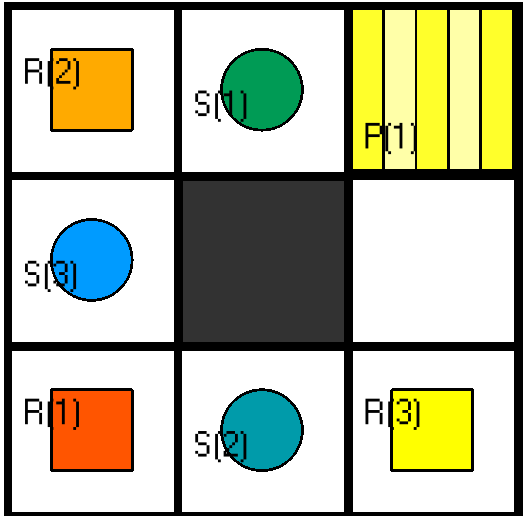
\includegraphics[width=75mm]{Images/Instance 1}
\caption{Benchmark\_1 by Tarek Ramadan}
\label{fig:I1}
\end{figure}

\begin{figure}[h]
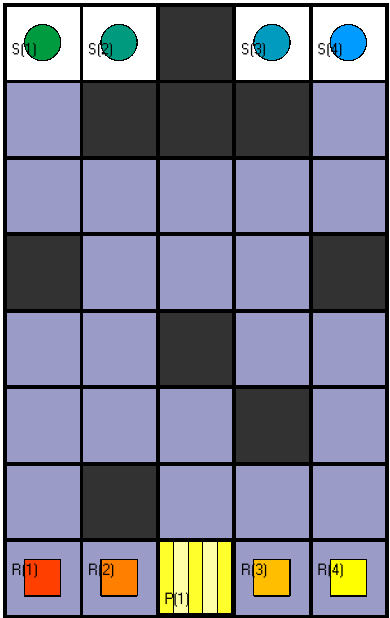
\includegraphics[width=75mm]{Images/Instance 2}
\caption{Benchmark-5 by Marius W and Niklas K.}
\label{fig:I2}
\end{figure}

\begin{figure}[h]
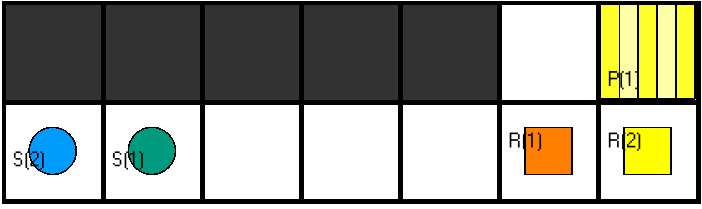
\includegraphics[width=75mm]{Images/Instance 3}
\caption{Instance 6 (Own Benchmark)}
\label{fig:I3}
\end{figure}


\section{Comparison with other Approaches}
There are 4 other groups that have worked on the same problem. In the appendix, the benchmark results of every solution can be found. For the group consisting of Marius Wawerek and Niklas Kämmer as well as the group consisting of Tom Schmidt, Hannes Weichelt and Jullian Bruns, I have used the python program created by the group of three. The program iteratively finds the minimal horizon for the used merger. \\
The solution of Tarek Ramadan \cite{github1} is able to solve most instances in a short time. The instances with 30 and 50 robots take too long for his solution as well. There are two instances his approach could not solve. Both of these were solvable by my approach. This means, his approach is generally faster but has problems with different instances. \\
The approach of Tom Schmidt, Hannes Weichelt and Julian Bruns \cite{github2} is very fast in the instances it can solve. It is the only approach that can solve the instances with 50 and 30 robots in the designated time frame. The downside is that there are three instances that are unsatisfiable. Benchmark\_1 (the circular shape) is one of them. Another unsolvable instance is the one where the robots have to move away from their original path together which seems to be a problem for this approach. The third unsatisfiable instance is a rather simple problem with only one conflict which makes it weird that it cannot be solved. The approach of this group seems to be very fast. The downside to it is that it cannot solve some instances.  \\
The solution of Marcus Funke and Maximilian Wiedenhöft \cite{github3} seems to have problems similar to mine. It is very time inefficient. Furthermore, there are three instances that cannot be solved. One of those instances is Benchmark\_1 which my approach could not solve either. Their solution can however solve the other instance mine could not. To summarize, their approach is time inefficient as well and there is a similar amount of instances it cannot solve. \\
The solution of Marius Wawerek and Niklas Kämmer \cite{github4} has very short solution times for most instances. The only instances that could not be solved in the designated time were the ones with 30 and 50 robots. There is no instance that is unsolvable. It seems to be the best solution for solving small instances. There does not seem to be any instance it cannot solve. The only problem is that the solving time rises too high if there are too many robots.

\section{Conclusion}
This paper explained my approach on how to solve the plan merging problem for the asprilo framework. The solution is able to solve almost all of the benchmarks with the exception being two very niche 
benchmarks that are unlikely to appear in the real world. There are two main problems in my solution. The first is that it is very time inefficient. The second is that the user has to input the time horizon and
the maximum conflict number. If he does not know it, he will likely take an upper bound which increases the computation time. While those two problems are definitely a major deficit of my solution, the trade-off
is that it is generally usable and it finds a solution with the minimum amount of conflicts needed to solve a problem instance. 
This means that it can be used in small instances where there are not two many robots and a small amount of conflicts.\\
My solution to solving the plan merging problem has a lot of possibilities of getting improved, like time efficiency and taking it to the A-domain of the framework. Nevertheless, it is an approach that solves the problem and could
be used in certain scenarios.

\newpage

\begin{thebibliography} {6}
\bibitem{asprilo}
asprilo framework
\begin{verbatim}
https://asprilo.github.io/
\end{verbatim}

\bibitem{owngithub}
My Github Repository
\begin{verbatim}
https://github.com/salewsky/Plan-Merging
\end{verbatim}

\bibitem{github1}
Github Repository of Tarek Ramadan
\begin{verbatim}
https://github.com/tramadan-up/asprilo-project
\end{verbatim}

\bibitem{github2}
Github Repository of Tom Schmidt, Hannes Weichelt and Julian Bruns
\begin{verbatim}
https://github.com/tzschmidt/PlanMerger
\end{verbatim}

\bibitem{github3}
Github Repository of Marcus Funke and Maximilian Wiedenhöft
\begin{verbatim}
https://github.com/Zard0c/ProjektMAPF
\end{verbatim}

\bibitem{github4}
Github Repository of Marius Wawerek and Niklas Kämmer
\begin{verbatim}
https://github.com/NikKaem/mapf-project
\end{verbatim}

\end{thebibliography}

\newpage
\appendix
\section{Benchmark Results}
The solver was interrupted after a solving time of half an hour. If the solver needed more time than that,
the solving time is shown as ``TOO LONG''. The solver did not find a solution if these instances were tested with smaller parameters. The instances that were ``UNSATISFIABLE'' are the ones that are unlikely to return a solution even when using
higher parameters. ``Unlikely'' means that the approach the group took is not able to theoretically solve the instance. 

\subsection{My Solver}
\begin{tabular}[h]{l|c|c|c|c|c}
Instance & Time & CPU-Time & Horizon & Solved Conflicts & Robots \\
Instance 1 & 0.125s & 0.109s & 5 & 1 & 2 \\
Instance 5 & 0.484s & 0.469s & 4 & 3 & 4 \\
Instance 6 & 696.239s & 695.594s & 14 & 9 & 2 \\
Instance 7 & 134.847s & 134.672 & 9 & 3 & 8 \\
bench\_test\_2 & 0.125s & 0.109s & 7 & 1 & 2 \\
bench\_test\_3 & 0.078s & 0.063s & 4 & 1 & 2 \\
bench\_test\_16\_mod1 & 11.220s & 10.922s & 8 & 5 & 4 \\
Benchmark-5 & \multicolumn{2}{c|}{UNSATISFIABLE(1525s)} & 17 & 14 & 4 \\
Benchmark-6 & 881.982s & 875.938s & 10 & 6 & 8 \\
Benchmark-42 & 16.619s & 16.531s & 10 & 1 & 5 \\ 
Benchmark-51 & 1702.764s & 1696.922s & 23 & 1 & 6 \\
Benchmark 03 & 16.467s & 16.188s & 7 & 5 & 4 \\
Benchmark 05 & 0.121s & 0.094s & 4 & 1 & 3 \\
Benchmark R1 &\multicolumn{2}{c|}{TOO LONG} & 20 & 1 & 50 \\
Benchmark R2 & \multicolumn{2}{c|}{TOO LONG} & 20 & 1 & 30 \\
Benchmark\_1 & \multicolumn{2}{c|}{UNSATISFIABLE(355s)} & 8 & 8 & 3 \\ 
Benchmark\_2 & \multicolumn{2}{c|}{TOO LONG} & 19 & 10 & 2 \\
Benchmark\_3 & 1.075s & 1.063s & 9 & 2 & 3 \\
Benchmark\_4 & 3.133s & 3.109s & 15 & 4 & 2 \\
\end{tabular}

\subsection{Tarek Ramadan}
\begin{tabular}[h]{l|c|c|c|c|c}
Instance & Time & CPU-Time & Horizon & Constant rm & Robots \\
Instance 1 & 0.172s & 0.141s & 5 & 1 & 2 \\
Instance 5 & \multicolumn{2}{c|}{UNSATISFIABLE(0.06s)} & - & 10 & 4 \\
Instance 6 & 0.246s & 0.234s & 14 & 9 & 2 \\
Instance 7 & \multicolumn{2}{c|}{UNSATISFIABLE(5.88s)} & - & 10 & 8 \\
bench\_test\_2 & 0.159s & 0.109s & 5 & 2 & 2 \\
bench\_test\_3 & 0.134s & 0.125s & 4 & 3 & 2 \\
bench\_test\_16\_mod1 & 0.241s & 0.203s & 6 & 4 & 4 \\
Benchmark-5 & 0.762s & 0.688s & 17 & 7 & 4 \\
Benchmark-6 & 1.213s & 1.063s & 11 & 5 & 8 \\
Benchmark-42 & 1.673s & 1.578s & 11 & 2 & 5 \\ 
Benchmark-51 & 13.101s & 11.891s & 23 & 3 & 6 \\
Benchmark 03 & 0.266s & 0.172s & 5 & 4 & 4 \\
Benchmark 05 & 0.142s & 0.094s & 4 & 3 & 3 \\
Benchmark R1 &\multicolumn{2}{c|}{TOO LONG} & - & 5 & 50 \\
Benchmark R2 & \multicolumn{2}{c|}{TOO LONG} & - & 5 & 30 \\
Benchmark\_1 & 0.219s & 0.156s & 5 & 4 & 3 \\ 
Benchmark\_2 & 1.687s & 1.516s & 19 & 16 & 2 \\
Benchmark\_3 & 0.904s & 0.734s & 14 & 6 & 3 \\
Benchmark\_4 & 0.298s & 0.281s & 15 & 8 & 2 \\
\end{tabular}

\subsection{Tom Schmidt, Hannes Weichelt and Julian Bruns}
\begin{tabular}[h]{l|c|c|c}
Instance & Solving Time & Horizon & Robots \\
Instance 1 & 0.066s & 5 & 2 \\
Instance 5 & 0.060s  & 3 & 4 \\
Instance 6 & 0.110s & 8 & 2 \\
Instance 7 & 0.851s  & 10 & 8 \\
bench\_test\_2 & UNSATISFIABLE(60s) & 20 & 2 \\
bench\_test\_3 & 0.071s & 6 & 2 \\
bench\_test\_16\_mod1 & 0.231s & 8 & 4 \\
Benchmark-5 & 0.474s & 13 & 4 \\
Benchmark-6 & 3.409s & 13 & 8 \\
Benchmark-42 & 0.112s & 11 & 5 \\ 
Benchmark-51 & 1.712s & 23 & 6 \\
Benchmark 03 & 0.192s & 7 & 4 \\
Benchmark 05 & 0.045s & 5 & 3 \\
Benchmark R1 & 184.887s & 23 & 50 \\
Benchmark R2 & 255.805s & 62 & 30 \\
Benchmark\_1 & UNSATISFIABLE(5s) & 15 & 3 \\ 
Benchmark\_2 & UNSATISFIABLE(83s) & 25 & 2 \\
Benchmark\_3 & 0.212s & 11 & 3 \\
Benchmark\_4 & 0.437s & 15 & 2 \\
\end{tabular}




\subsection{Marcus Funke and Maximilian Wiedenhöft}
\begin{tabular}[h]{l|c|c|c|c}
Instance & Time & CPU-Time & Horizon &  Robots \\
Instance 1 & 1.672s & 1.656s & 5 & 2 \\
Instance 5 & \multicolumn{2}{c|}{UNSATISFIABLE(42s)} & 10 & 4 \\
Instance 6 & 9.947s & 9.766s & 14 & 2 \\
Instance 7 & \multicolumn{2}{c|}{TOO LONG} & 9  & 8 \\
bench\_test\_2 & 3.361s & 3.172s & 7 & 2 \\
bench\_test\_3 & 0.437s & 0.422s & 4 & 2 \\
bench\_test\_16\_mod1 & 20.751s & 20.703s & 9 & 4 \\
Benchmark-5 & 1398.237s & 1347.656s & 17 & 4 \\
Benchmark-6 & \multicolumn{2}{c|}{TOO LONG} & 13 & 8 \\
Benchmark-42 & \multicolumn{2}{c|}{TOO LONG} & 10  & 5 \\ 
Benchmark-51 & \multicolumn{2}{c|}{TOO LONG} & 23 & 6 \\
Benchmark 03 & 22.019s & 21.438s & 7 & 4 \\
Benchmark 05 & 0.547s & 0.531s & 4 & 3 \\
Benchmark R1 &\multicolumn{2}{c|}{TOO LONG} & 25 & 50 \\
Benchmark R2 & \multicolumn{2}{c|}{TOO LONG} & 25 & 30 \\
Benchmark\_1 & \multicolumn{2}{c|}{UNSATISFIABLE(5s)} & 10 & 3 \\ 
Benchmark\_2 & \multicolumn{2}{c|}{UNSATISFIABLE(56s)} & 25 & 2 \\
Benchmark\_3 & 92.768s & 92.250s & 10 & 3 \\
Benchmark\_4 & 26.482s & 26.422s & 16 & 2 \\
\end{tabular}

\subsection{Marius Wawerek and Niklas Kämmer}
\begin{tabular}[h]{l|c|c|c}
Instance & Solving Time & Horizon & Robots \\
Instance 1 & 0.049s & 5 & 2 \\
Instance 5 & 0.060s  & 3 & 4 \\
Instance 6 & 0.065s & 6 & 2 \\
Instance 7 & 0.517s  & 9 & 8 \\
bench\_test\_2 & 0.064s & 5 & 2 \\
bench\_test\_3 & 0.046s & 4 & 2 \\
bench\_test\_16\_mod1 & 0.075s & 6 & 4 \\
Benchmark-5 & 0.794s & 11 & 4 \\
Benchmark-6 & 0.534s & 9 & 8 \\
Benchmark-42 & 0.723s & 10 & 5 \\ 
Benchmark-51 & 0.577s & 21 & 6 \\
Benchmark 03 & 0.078s & 5 & 4 \\
Benchmark 05 & 0.038s & 4 & 3 \\
Benchmark R1 & TOO LONG & 23 & 50 \\
Benchmark R2 & TOO LONG & 57 & 30 \\
Benchmark\_1 & 0.087 & 7 & 3 \\ 
Benchmark\_2 & 1.575s & 19 & 2 \\
Benchmark\_3 & 0.201s & 9 & 3 \\
Benchmark\_4 & 0.269s & 15 & 2 \\
\end{tabular}

\end{document}